% !TEX encoding = UTF-8 Unicode
% !TeX spellcheck = fr_FR
\documentclass[12pt,twoside,a4paper]{article}

% décommenter si nessecaire !TeX TXS-program:compile = txs:///pdflatex/[--shell-escape]
%\usepackage{minted}


\title{Filtre de Kalman}
\author{Sarah Curtit}
\date{}

\usepackage[dvipsnames]{xcolor}
\usepackage{amsfonts}
\usepackage{amsmath}
\usepackage{amssymb}
\usepackage{amsthm}
\usepackage[french]{babel}
\usepackage{beramono}
\usepackage{changepage}
\usepackage{color}
\usepackage{mathdots}
\usepackage[utf8]{inputenc}
\usepackage{enumitem}
\usepackage{fancyhdr}
\usepackage{float}
\usepackage{framed}
\usepackage[T1]{fontenc}
\usepackage[margin=1in]{geometry}
\usepackage{listings}
\usepackage{mathrsfs}
\usepackage{tikz, tkz-tab}
\usepackage[european resistor]{circuitikz}
\usepackage{titling}
\usepackage{tabularx}
\usepackage{graphicx}
\usepackage{textcomp}
\usepackage{gensymb} %en tant que le package 'was'
\usepackage{physics}
\usepackage{marvosym}
\usepackage{standalone}
\usepackage{preview}
\usepackage{mathtools}
\usepackage[hidelinks]{hyperref}
\hypersetup{allcolors=black}


\usetikzlibrary{decorations.pathmorphing,patterns}

\newtheoremstyle{dotless}{}{}{\itshape}{}{\bfseries}{}{ }{}
\theoremstyle{dotless}

\newtheorem{defs}{D\'efinition}[subsection]
\newenvironment{defi}{\definecolor{shadecolor}{RGB}{255,236,217}\begin{shaded}\begin{defs}\ \\}{\end{defs}\end{shaded}}

\newtheorem{pro}{Propri\'et\'e}[subsection]
\newenvironment{prop}{\definecolor{shadecolor}{RGB}{230,230,255}\begin{shaded}\begin{pro}\ \\}{\end{pro}\end{shaded}}

\newtheorem*{theos}{Th\'eor\`eme}
\newenvironment{theo}[1]{\definecolor{shadecolor}{RGB}{230,230,255}\begin{shaded}\begin{theos}\textbf{\emph{#1}}\ \\}{\end{theos}\end{shaded}}

\newtheorem{cor}{Corollaire}[subsection]
\newenvironment{coro}{\definecolor{shadecolor}{RGB}{245,250,255}\begin{shaded}\begin{cor}\ \\}{\end{cor}\end{shaded}}

\setlength{\droptitle}{-1in}
%\predate{}
%\postdate{}
%\title{\textbf{\titre}\\\soustitre\vspace{-.18in}}

\pagestyle{fancy}
\makeatletter
\lhead{\title}
\rhead{\@author}
\makeatother

\newenvironment{preuve}{\begin{framed}\begin{proof}[\unskip\nopunct]}{\end{proof}\end{framed}}
\newenvironment{liste}{\begin{itemize}[leftmargin=*,noitemsep, topsep=0pt]}{\end{itemize}}
\newenvironment{tab}{\begin{adjustwidth}{.5cm}{}}{\end{adjustwidth}}

\newcommand{\lbracket}{[\![}
\newcommand{\rbracket}{]\!]}
\newcommand{\fonction}[5]{\begin{aligned}[t]#1\colon#2&\longrightarrow#3 \\#4&\longmapsto#5\end{aligned}}
\newcommand{\systeme}[1]{\left\{\begin{aligned}#1\end{aligned}\right.}
\newcommand{\cercle}[1]{\textcircled{\scriptsize{#1}}}
\newcommand{\Sup}{\mathop{\text{Sup}}}
\newcommand{\Inf}{\mathop{\text{Inf}}}
\newcommand{\lf}[1]{\left(#1\right)}
%\newcommand{\C}{\mathbb{C}}
\newcommand{\R}{\mathbb{R}}
\newcommand{\K}{\mathbb{K}}
\newcommand{\Q}{\mathbb{Q}}
\newcommand{\N}{\mathbb{N}}
\newcommand{\Z}{\mathbb{Z}}
\newcommand{\I}{\mathcal{I}}
\newcommand{\F}{\mathcal{F}}
\newcommand{\E}{\mathcal{E}}
%\newcommand{\G}{\mathcal{G}}
\newcommand{\et}{\text{ et }}
\newcommand{\ou}{\text{ ou }}
\newcommand{\xou}{\ \fbox{\text{ou}}\ }
\newcommand{\vdashv}{\mathrel{\text{\ooalign{$\vdash$\cr$\dashv$\cr}}}}
\newcommand{\card}{\text{card}}
\newcommand{\restr}[2]{{% we make the whole thing an ordinary symbol
		\left.\kern-\nulldelimiterspace % automatically resize the bar with \right
		#1 % the function
		\vphantom{\big|} % pretend it's a little taller at normal size
		\right|_{#2} % this is the delimiter
	}}
\newcommand{\floor}[1]{\lfloor #1 \rfloor}
\newcommand{\ceil}[1]{\lceil #1 \rceil}
\newcommand{\Sev}{\mathrm{S}_\mathrm{EV}}
\newcommand{\vect}{\mathrm{Vect}}
\newcommand{\Kev}{\K_\mathrm{EV}}

%%
%% Julia definition (c) 2014 Jubobs
%%
\lstdefinelanguage{Julia}%
{
	morekeywords={abstract,break,case,catch,const,continue,do,else,elseif,%
		end,export,false,for,function,immutable,import,importall,if,in,%
		macro,module,otherwise,quote,return,switch,true,try,type,typealias,%
		using,while},%
	sensitive=false,%
	alsoother={$},%
	morecomment=[l]\#,%
	morecomment=[n]{\#=}{=\#},%
	morestring=[s]{"}{"},%
	morestring=[m]{'}{'},%
}[keywords,comments,strings]%

%%
%% Laplacien et D'Alembertien
%%
\newcommand*\Laplace{\mathop{}\!\mathbin\bigtriangleup}
\newcommand*\DAlambert{\mathop{}\!\mathbin\Box}

\usepackage[utf8]{inputenc}

\newcommand\ul[1]{\underline{#1}}
\newcommand\ull[1]{\underline{\underline{#1}}}
%\usepackage{minted}



\begin{document}
	\maketitle
	
\section{Presentation du Filtre de Kalman}

\subsection{Le filtre de Kalman continu}

\subsubsection{Le modèle}
	
Le filtre de Kalman est un modèle d'état défini par deux équations: 

$$
\left\{ 
\begin{array}{ll}
        \dot{x}(t) = A x(t)  + B u(t) +M w(t)  & \text{équation d'état}  \\
        y(t) = C x(t) + Du(t) + v(t) & \text{équation de mesure} 
\end{array}
\right.
$$



x est un vecteur d'état, y un vecteur de mesures, u un vecteur de commandes (données déterminées), tandis que les signaux $w(k)$ et $v(k)$ sont des bruits blancs gaussiens centrés de densité spectrale de puissance $W$ et $V$ respectivement. On a 
$$
\begin{array}{lll}
E[w(k) w(k+l)^T ] &= W\delta(l) & \delta(l) \text{ = 1 si l=0; 0 sinon} \\
E[v(k) v(k+l)^T ] &= V \delta(l) & \text{(V doit être inversible)}\\
E[w(k) v(k+l)^T ] &= 0 & \\
\end{array}
$$

\subsubsection{Minimisation de l'erreur d'estimation} 

En pratique, le filtre doit retourner en sortie l'état estimé du système, noté $\hat{x}$.
L'équation d'état du filtre nous est donnée par 
$$ \hat{\dot{x}}(t) = A_f\hat{x}(t)+B_fu(t)+K_fy(t) $$
où $A_f$ $B_f$ et $K_f$ sont des matrices à déterminer. \\
\vspace{0.5cm}

\noindent Soit $\varepsilon(t)= x(t)-\hat x(t)$ l'erreur d'estimation du système. On souhaite que cet estimateur soit non biaisé, c'est à dire que $\lim\limits_{t \rightarrow +\infty } \bar{\varepsilon}= 0 $ quel que soit le profil de commande et quel que soit l'état initial ($\bar{\varepsilon}$ étant l'espérance mathématique de $\varepsilon$). 
\vspace{0.5cm}\\
L'écriture de ces conditions nous donne finalement l'équation du filtre de Kalman 
$$
\hat{\dot{x}}(t) = (A\hat x + Bu) + K_f (y -C \hat x -Du)
$$
$K_f$ est appelé le gain du filtre. C'est lui qui traduit la confiance que l'on a dans le modèle ou les mesures. Si on considère que le modèle est très fiable et les mesures très bruitées on accordera peu d'importance à celles-ci, et $K_f$ sera petit. Si l'on fait au contraire plus confiance aux mesures qu'au modèle, $K_f$ sera grand. 
\vspace{1cm}

Afin d'obtenir le filtre le plus fiable possible, le gain $K_f$ doit minimiser la variance de l'erreur d'estimation, c'est à dire la trace de la matrice de covariance de l'erreur d'estimation, 
$$
\begin{array}{lll}
P(t) &=& E[(x(t)-\hat x(t))(x(t)-\hat x(t))^T] \\
\end{array}
$$ 

$P(t)$ vérifiant l'équation
$$ 
\dot{P}(t) = (A-K_{f}C)P(t)+P(t)(A-K_{f}C)^{T} + MWM^{T} + K_{f}VK_{f}^{T}
$$

En minimisant P on obtient
$$
\begin{array}{lll}
K_f &=& P(t)C^T V^{-1} \\
\dot{P}(t) &= &AP(t) +P(t)A^T -P(t)C^TV^{-1}CP(t)+MWM^T
\end{array}
$$

Cette deuxième équation étant appelée équation différentielle de Riccati.
\vspace{1cm}

Une fois les erreurs d'initialisation corrigées (régime constant), on obtient 
$$
\begin{array}{llll}
K_f &=& P(t)C^T V^{-1} &\text{Désormais constant.}\\ 
0 &= &AP(t) +P(t)A^T -P(t)C^TV^{-1}CP(t)+MWM^T & \text{P étant la solution positive de l'équation.}
\rule[0pt]{0mm}{15pt} \\
\end{array}
$$



\subsection{Le filtre de Kalman discret}

\subsubsection{Le modèle}
Dans les faits, les appareils numériques fonctionnent de manière discrète. \\
On utilisera donc en pratique le modèle de Kalman discret
$$
\left\{ 
\begin{array}{lll}
        x(k+1) = A_d x(k) + B_d u(k) +M_d w_d(k) & \text{équation d'état} & x \in \mathbb{R}^n, y \in \mathbb{R}^m, w_d \in \mathbb{R}^q\\
       y(k) = C_d x(k) + Du(k) + v_d(k) & \text{équation de mesure} & y \in \mathbb{R}^m, v_d \in \mathbb{R}^p\\
\end{array}
\right.
$$

Les signaux $w_d$ et $v_d$ sont cette fois associés à des matrices de covariance $W_d$ et $V_d$ telles que
$$
\begin{array}{lll}
E[w_d(k) w_d(k+l)^T ] &= W_d \delta(l) &  \\
E[v_d(k) v_d(k+l)^T ] &= V_d \delta(l) & \text{($V_d$ doit être inversible)}\\
E[w_d(k) v_d(k+l)^T ] &= 0 & \\
\end{array}
$$
On note $dt$ le pas de temps associé au système discret.\\

\subsubsection{Passage du modèle continu au modèle discret}

\vspace{0.3cm}
Le modèle de Kalman discret est très proche du modèle continu, et on peut obtenir les nouvelles matrices discrètes à partir de celles du modèle continu. On a
$$ \begin{array}{ccccc}
A_d = e{Adt} \rule[0pt]{30pt}{0pt}
B_d = \int_0^{dt} e^{Av}Bdv \, \mathrm{d}v \rule[0pt]{30pt}{0pt}& 
M_d = I_n \rule[0pt]{30pt}{0pt}&
C_d = C\rule[0pt]{30pt}{0pt} & 
V_d= \frac{V}{dt}\rule[0pt]{30pt}{0pt}\\
\end{array} $$

\noindent L'expression de $W_d$ est plus compliquée puisqu'on a $W_d = \int_0^{dt}e^{Av}MWM^Te^{A^T v} \, \mathrm{d}v$ \\
Cependant dans l'hypothèse où $dt$ est petit par rapport au temps de réponse du système, on peut écrire
$$ W_d \approx dtMWM^T$$ 

\subsubsection{Représentation d'état, implémentation du filtre en pratique}


Comme dans le modèle continu, on souhaite optimiser le gain $K_{f}$ afin de minimiser l'erreur d'estimation. \\
Dans la suite de cette section, on distinguera 
$$
\begin{array}{ll}
	\begin{array}[t]{l}
	\text{l'état prédit à l'instant k+1}\\
	\text{connaissant toutes les mesures jusqu'à l'instant k} 
	\end{array} & \hat x(k+1|k) \\
	
	\begin{array}{l}
	\text{l'état estimé connaissant la mesure à l'instant k+1 (après recalage)} 
	\end{array} & \hat x(k+1|k+1) \rule{0pt}{15pt}
\end{array}
$$ 

\noindent L'état prédit est calculé de fa\c con déterministe
$$ \hat x(k+1|k) = A_{d} \hat x (k|k) +B_du(k)$$

\noindent Tandis que l'équation d'état du filtre 
$$ \hat{\dot{x}}(k|k) = A_d\hat{x}(k|k)+B_du(k)+K_f(k+1)\big(y(k) - C_{d} \hat x(k|k) - D \hat x(k|k) \big) $$
\indent nous donne 
$$ \hat x(k+1|k+1) = \hat x(k+1|k)+ K_{f}(k+1)\big(y(k) - C_{d} \hat x(k|k) - D \hat x(k|k) \big)$$

La combinaison de ces deux équations nous permet d'obtenir la représentation d'état du filtre de Kalman permanent: 
$$
\boxed{
\left\{
\begin{array}{lll}
\hat x(k|k) &=& (I-K_f C_d)\hat x(k|k-1)+
	\begin{pmatrix} K_f & -K_f D \end{pmatrix}
	\begin{pmatrix} y(k) \\ u(k) \end{pmatrix} \\
\hat x( k+1|k) &=& A_d(I-K_f C_d) \hat x (k|k-1) + 
	\begin{pmatrix} A_d K_f & B_d-A_dK_fD \end{pmatrix}
	\begin{pmatrix} y(k) \\ u(k)\end{pmatrix} \\
\end{array}
\right.}
$$

\noindent C'est la deuxième équation, calculant l'état prédit à l'instant k+1 qui nous intéresse et qui sera implémenté dans l'algorythme du filtre de Kalman. \\

\vspace{1cm} 

Afin de totalement déterminer cette équation, il reste cependant à déterminer $K_{f}$, choisi encore une fois afin de minimiser l'erreur d'estimation $P(k+1|k+1)$ (dont l'expression est extrêmement compliquée).

La résolution de l'équation différentielle nous donne 
$$
\begin{array}{lll}
K_{f}(k+1) &=& P(k+1|k)C_{d}^{T}(C_{d}P(k+1|k)C_{d}^{T}+V_{d})^{-1} \\
P(k+1|k) &=&  A_{d}P(k|k-1)A_{d}^{T} -A_{d}P(k|k-1)C_{d}^{T}\big(C_{d}P(k|k-1)C_{d}^{T}+V_{d}\big)^{-1}C_{d}P(k|k-1)A_{d}^{T} \\
&& + M_{d}W_{d}M_{d}^{T}
\end{array}
$$

En régime permanent la matrice de covariance de l'erreur de prédiction est constante et vérifie l'équation discrète de Riccati
$$ P_{p} =  A_{d}P_{p}A_{d}^{T} -A_{d}P_{p}C_{d}^{T}\big(C_{d}P_{p}C_{d}^{T}+V_{d}\big)^{-1}C_{d}P_{p}A_{d}^{T}  + M_{d}W_{d}M_{d}^{T} $$

\vspace{1cm} 
On peut en déduire le gain du filtre et la matrice de covariance de l'erreur d'estimation 
$$ 
\begin{array}{lll}
K_{f} &=& P_{p}C_{d}^{T}(C_{d}P_{p}C_{d}^{T}+V_{d})^{-1} \\
P_{e} &=& (I-K_{f}C_{d})P_{p}
\end{array}$$



La plupart des solveurs actuels proposent des fonctions permettant de résoudre l'équation de Riccati. 
Dans le cadre de ce projet, nous avons travaillé avec Python et la fonction scipy.linalg.solve\_discrete\_are. \\

\section{Application au problème}

\subsection{Problème 1D}

Pour simplifier le problème, considérons tout d'abord que l'outil utilisé est parfaitement perpendiculaire à la surface au point de contact et qu'il n'y a pas de frottement. Dans ce cas, on peut se permettre de considérer seulement les données selon z (repère orienté selon la normale à la surface au point courant).

On prend alors comme vecteurs d'état et de mesure respectivement
$$
\begin{array}{ccc}
x =  \begin{pmatrix} z & \dot{z} \end{pmatrix} 
,   & 
y= \begin{pmatrix}
 F_z \
\end{pmatrix},   &
u = \underline{0}
\end{array}
$$

ce qui simplifie grandement le problème

\vspace{1cm}




v et w sont ici respectivement le vecteur des signaux aléatoires qui polluent les mesures y et le vecteur  des signaux inconnus qui viennent perturber directement l'équation d'état du système. Ici  v représente l'imprécision du capteur et w rend compte des aspérités de la surface et de l'imprécision du robot. \\
La matrice M relie le bruit d'état $w_x$ à w par la relation $w_x = Mw$

\noindent
En faisant pour l'instant abstraction des vecteurs d'erreurs (et donc du dernier terme de chaque égalité) le système s'écrit dans notre cas comme  

$$
\left\{ 
\begin{array}{ll}
        \begin{pmatrix} \dot{z} \\ \ddot{z} \end{pmatrix} 
        &= \begin{pmatrix}
        0 & 1 \\
        0 & 0 \\ 
        \end{pmatrix}.
        \begin{pmatrix} z  \\ \dot{z} \end{pmatrix} \\
        \vspace{0.5cm} \\
        \begin{pmatrix} F_z  \end{pmatrix}
         &= \begin{pmatrix} 
         k & 0
	\end{pmatrix}.
	 \begin{pmatrix} z \\  \dot{z} \end{pmatrix} \\
\end{array}
\right.
$$

Expliquons ce modèle. \\
La matrice A est déterminée à l'aide du premier principe de Newton. Celui-ci nous donne l'équation
$ ma_z = k*(dz) $, où m est la masse totale du système et k est la raideur du ressort (on néglige toujours les frottements)
\\
La matrice C est elle déterminée à partir d'une simple loi de Hooke: $F_z = k*d_z$. 

\vspace{2cm}

Déterminons désormais les  matrices associées vecteurs d'erreur v et w. \\
on note 
$$
\begin{array}{lll}
 v &= \begin{pmatrix} v_{z} & v_{\dot{z}}  \end{pmatrix} ^T  & \text{où $v_z$ représente l'incertitude sur $F_z$} \\
 w &= \begin{pmatrix} w_z & w_{\dot{z}} &  w_{\delta{z}} \end{pmatrix}^T & 
 		\text{où}
		\begin{array}[t]{l}
		\text{$w_z$ représente l'incertitude de position du robot selon z} \\
		\text{$w_{\dot{z}}$ représente l'incertitude de vitesse selon z} \\
		\text{$w_{\delta{z}}$ représente l'incertitude sur les aspérités de la surface} \\
		\end{array} \\

 \end{array}
 $$
 


w(t) et v(t) sont des vecteurs gaussiens centrés de densité spectrale de puissance W et V respectivement. On a :

$$
\begin{array}{ll}
E[w(t) w(t+\tau)^T ] &= W \delta(\tau) \\
E[v(t) v(t+\tau)^T ] &= V \delta(\tau)  \\
E[w(t) v(t+\tau)^T ] &= 0  \\
\end{array}
$$

\vspace{1cm}

V peut-être calculé à partir des données d'échantillonnage du capteur. On a en effet les précisions suivantes:
$$
\begin{array}{|c|c|c|c|c|c|}	
	\hline
	\bold{F_x} & \bold{F_y} & \bold{F_z} & \bold{M_x} & \bold{M_y} & \bold{M_z} \\
	\hline 
	1.00\% & 1.25\% & 0.75\% & 1.00\% & 1.25\% & 1.50\% \\
	\hline
\end{array}
$$

On estime également les ordres de grandeur des forces et moments qui seront rencontrés par le capteur 
$$
\begin{array}{|c|c|c|c|c|c|}	
	\hline
	\bold{F_x} & \bold{F_y} & \bold{F_z} & \bold{M_x} & \bold{M_y} & \bold{M_z} \\
	\hline 
	1N & 1N & 20N & 1N.m & 1N.m & 1N.m \\
	\hline
\end{array}
$$

En notant $\delta F_z$ la précision de la force $F_z$ et $\overline{F_z}$ son ordre de grandeur on obtient

\hspace{-3mm}

\begin{align*}
V &= \begin{pmatrix}
\overline{F_z}^2\delta{F_z} - (\overline{F_z}\delta{F_z})^2
\end{pmatrix} \\
&=  \begin{pmatrix}
2.978
\end{pmatrix}
\end{align*}

%V &= \begin{pmatrix} Var(v_x) & Cov(v_x,v_y) & Cov(v_x,v_z) & Cov(v_x,v_{\dot{x}}) & Cov(v_x,v_{\dot{y}}) & Cov(v_x,v_{\dot{z}}) \\
%			      Cov(v_x,v_y) & Var(v_y) & Cov(v_y,v_z) & Cov(v_y,v_{\dot{x}}) & Cov(v_y, v_{\dot{y}}) & Cov(v_y,v_{\dot{z}}) \\
%			      Cov(v_x,v_z) & Cov(v_y,v_z) & Var(v_z) & Cov(v_z,v_{\dot{x}}) & Cov(v_z,v_{\dot{y}}) & Cov(v_z,v_{\dot{z}}) \\
%			      Cov(v_x,v_{\dot{x}}) & Cov(v_y, v_{\dot{x}}) & Cov(v_z, v_{\dot{x}}) & Var(v_{\dot{x}}) & Cov(v_{\dot{x}}, v_{\dot{y}}) & Cov(v_{\dot{x}}, v_{\dot{z}}) \\
%			      Cov(v_x, v_{\dot{y}}) & Cov(v_y, v_{\dot{y}}) &  Cov(v_z, v_{\dot{y}}) & Cov(v_{\dot{x}}, v_{\dot{y}}) & Var(v_{\dot{y}}) &  Cov(v_{\dot{y}}, v_{\dot{z}}) \\
%			      Cov(v_x, v_{\dot{z}}) & Cov(v_y, v_{\dot{z}}) & Cov(v_z, v_{\dot{z}}) & Cov(v_{\dot{x}}, v_{\dot{z}}) & Cov(v_{\dot{y}}, v_{\dot{z}}) & Var(v_{\dot{z}}) \\



\vspace{2cm}

On calcule ensuite W dont les termes diagonaux de la matrice sont les fonctions scalaires d'auto-corrélation de chaque composante du vecteur, tandis que les termes inter-diagonaux sont les fonctions d'inter-corrélation entre les différentes composantes. Les différentes composantes du vecteur étant indépendantes, W est une matrice diagonale.
$$
E[w(t) w(t+\tau)^T ] = W \delta(\tau) \\
$$


En considérant que la précision du robot est de 0,02mm en position ou en vitesse et que la précision de l'usinage de la surface est de 0,1mm, on en déduit W:

\begin{align*}
W &=
\begin{pmatrix}
0.02-0.02^2 & 0 & 0  \\
0 & 0.02-0.02^2  & 0  \\
 0 & 0 & 0.1-0.1^2  \\
\end{pmatrix} \\
&=
\begin{pmatrix}
0.0196 & 0 & 0  \\
0 & 0.0196 & 0  \\
0 & 0 & 0.09  \\
\end{pmatrix} \rule[20pt]{0pt}{10pt} 
\end{align*}


Déterminons enfin la matrice M qui permet de "relier" le vecteur w à ttl'équation d'état 
$$
M = 
\begin{pmatrix}
0 & 1 & 0 \\
\frac{k}{m} & 0 & \frac{k}{m}  \\
\end{pmatrix}
$$


Toutes les données de l'équation ayant été définies, on peut désormais calculer la matrice d'erreur P à partir de l'équation de Ricatti. 
$$ AP + PA^T -PC^T V^{-1} CP + MWM^{T} $$

Une résolution numérique nous donne 
$$
P = \begin{pmatrix} 0 & 0 \\
	0 & 0 
	\end{pmatrix} 
$$


\subsection{Modèle 2D}

Afin d'être plus réalistes, considérons désormais des forces selon les axes x et z, ainsi que le moment autours de l'axe y. Nous négligerons cependant toujours les frottements. \\

\begin{center}
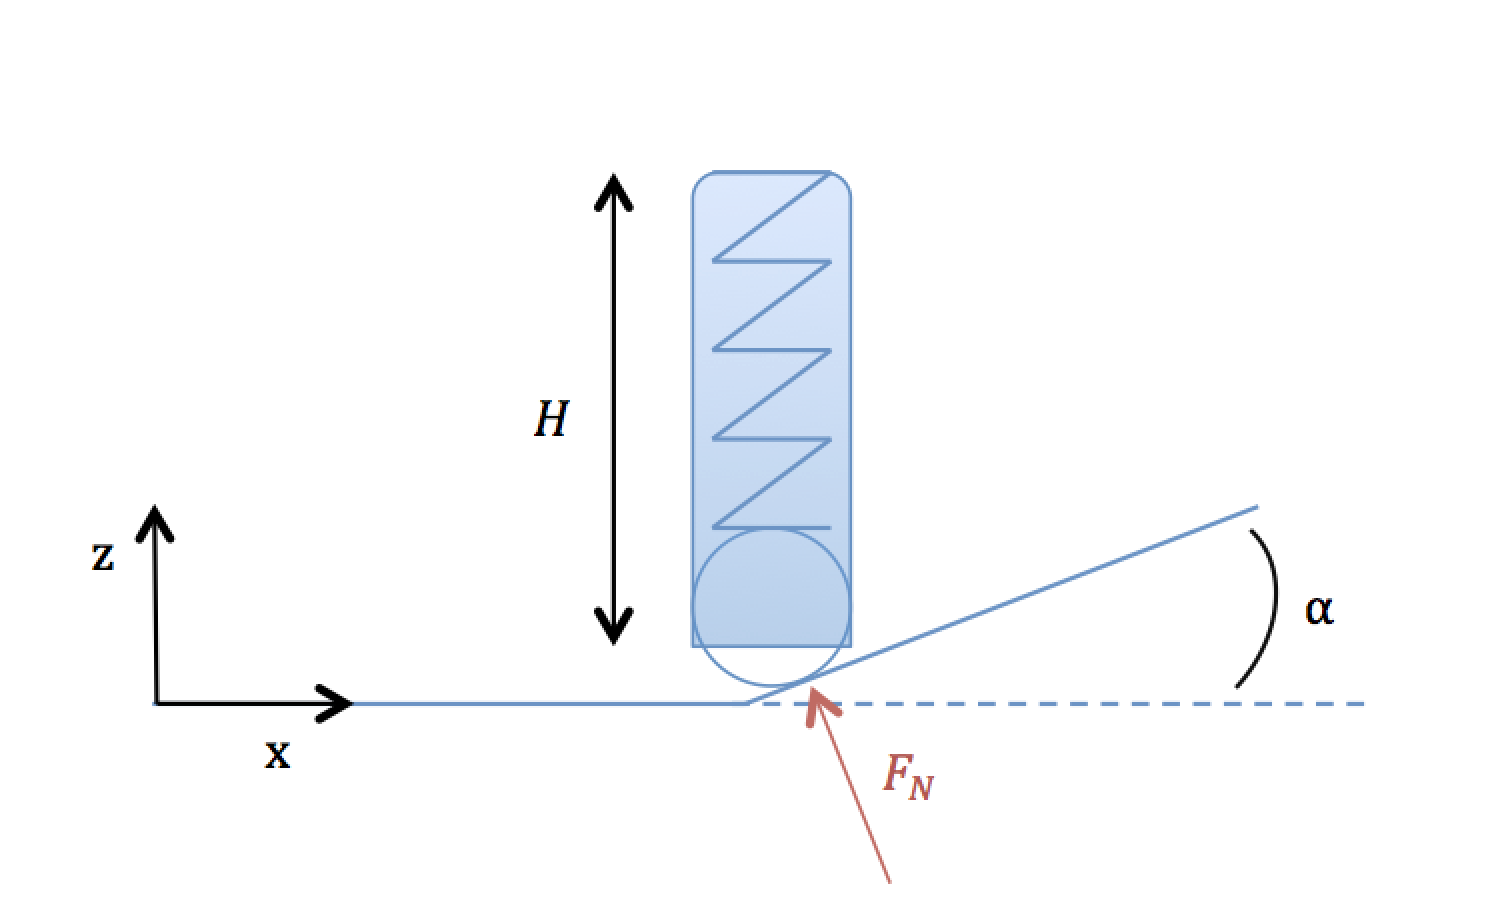
\includegraphics[scale=0.5]{schema_Kalman.png}
\end{center}


\vspace{1cm}
Plaçons nous dans le cas où l'outil n'est plus perpendiculaire à la surface (voir schéma ci-dessus)\\

Etant donné qu'il n'est pas possible de changer l'orientation du robot XXX -> CARO, nous nous bornerons toujours à corriger la trajectoire du robot. \\

\vspace{1cm}
Les valeurs mesurées par le capteur dépendent désormais de l'angle $\alpha$ formé avec l'horizontale. On a 

$$
\begin{array}{llll}
F_x &=& F_N sin(\alpha) &\\
F_z &=& F_N cos(\alpha) &\\
M_y &= &F_x*H &\\
	&= &F_N sin(\alpha)*H &
	\begin{array}[t]{l}
	\text{en faisant l'hypothèse que la hauteur découverte de la bille} \\ 
	\text{est négligeable devant la hauteur du poussoir}
	\end{array}
\end{array}
$$

L'objectif force devant désormais être mesuré selon la nouvelle normale à la surface, il convient de corriger en amont la valeur de $F_z$ injectée dans le filtre. 
On détermine tout d'abord $\alpha$ grâce aux données du capteur:
$$ \alpha = arctan(\frac{F_{x_c}}{F_{z_c}}) $$
On a 
$$
\begin{array}{lll}
F_{N_c} &=& \frac{F_{z_c}}{cos(\alpha)}  \\
F_N &=& F_{N_c}-F_{obj} \\
F_z &=& F_{z_c}-F_{obj}cos(\alpha)
\end{array}
$$

Afin de tenir compte de la pente imprévue, il faut également ajuster le déplacement et la vitesse selon z. \\
Pour cela, ..
$$ 
\begin{array}{lll}
u &=& (\dot{x}_{robot}) \\
D &=& \begin{pmatrix}
sin(\alpha)\\
0
\end{pmatrix} \\
\end{array}
$$
On 









\end{document}